\chapter{Filtros Digitales}

En este capítulo veremos como es el diseño de un filtro digital a partir de uno analógico, y para ello utilizaremos lo que se conoce como \textbf{Transformación Bilineal}. Esta transformación mapea el plano complejo del dominio de frecuencia analógico al dominio de frecuencia digital utilizando una relación no lineal.

Es importante tener en cuenta que la transformación bilineal introduce distorsiones en la respuesta en frecuencia del filtro analógico original al convertirlo en un filtro digital, como se muestra en la Figura \ref{fig:distorsion_frecuencia_angular}. Estas distorsiones son inevitables debido a la naturaleza no lineal de la transformación. Sin embargo, en muchos casos, estas distorsiones son aceptables y se pueden compensar mediante técnicas de diseño adicionales. Una de estas técnicas es el \textbf{Pre-Warping}.

\begin{figure}[H]
  \centering
  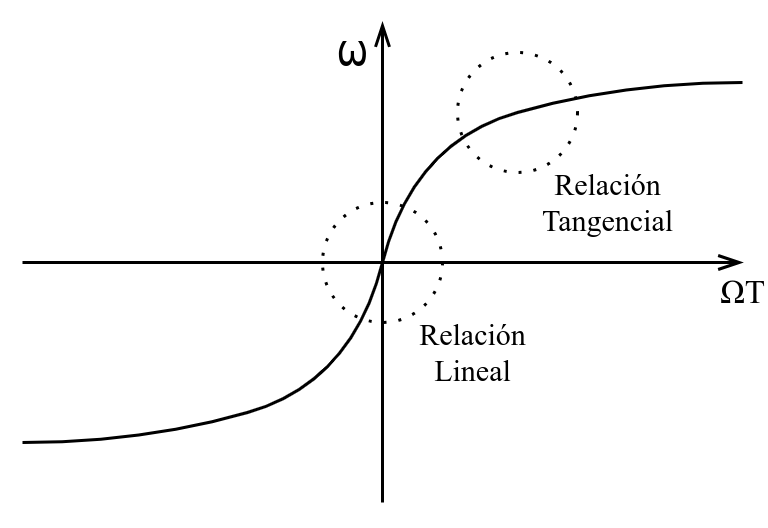
\includegraphics[width=300pt]{images/diagramas-distorsion-frecuencia.png}
  \caption{Distorsion de frecuencia introducida por la Transformación Bilineal}
  \label{fig:distorsion_frecuencia_angular}
\end{figure}

El pre-warping es un ajuste realizado a la \gls{fc} del filtro analógico antes de aplicar la transformación. Se hace con el fin de compensar la distorsión introducida por la transformación bilineal en las frecuencias más altas, esto es debido a la no linealidad de la función tangente utilizada en la transformación. El pre-warping ajusta la \gls{fc} del filtro analógico antes de aplicar la transformación bilineal para compensar esta distorsión. Se utiliza una función que aproxima la inversa de la función tangente para ajustar la \gls{fc} en el dominio analógico, como se muestra en la Ecuación \ref{eq:relacion_tangencial_frec_ang} \cite{rabiner1995theory}. Para más información acerca de la Transformación Bilineal se pueden consultar en las siguientes bibliografías: \cite{proakis1996digital}, \cite{oppenheim1989discrete} y \cite{oppenheim1999digital}.

\begin{equation}
  \Omega = \frac{2}{T} \tan \frac{\omega T}{2} = 2 f_s \tan\left(\pi \frac{f}{f_s}\right)
  \label{eq:relacion_tangencial_frec_ang}
\end{equation}


\section{Diseño}
Primero, se diseña el filtro analógico deseado utilizando un prototipo como el filtro Butterworth, Chebyshev o el Elíptico. En este caso usaremos el filtro Butterworth, que se caracteriza por tener una respuesta en frecuencia lo más plana y suave posible en la banda de paso, lo que significa que atenúa las frecuencias no deseadas de manera gradual y sin oscilaciones abruptas, como describre la Figura \ref{fig:diagrama_bode_pasa_bajos}.

El filtro de Butterworth más típico es el filtro pasa bajo de primer orden, el cual puede ser modificado a un filtro pasa banda a traves transformaciones que veremos más adelante, o añadir en serie otros formando un filtro pasa banda o elimina banda y filtros de mayores órdenes. La función transferencia para un filtro prototipo Butterworth pasa-bajos que corta en 1rad/s se describe en la Ecuación \ref{eq:butter_lp_norm}. Si deseamos diseñar un filtro pasa-altos, o pasa-banda o de rechaza-banda, basta con partir del filtro paso bajo prototipo y realizar una transformación en frecuencia.

\begin{equation}
  H(s) = \frac{1}{s+1}
  \label{eq:butter_lp_norm}
\end{equation}

\begin{figure}[H]
  \centering
  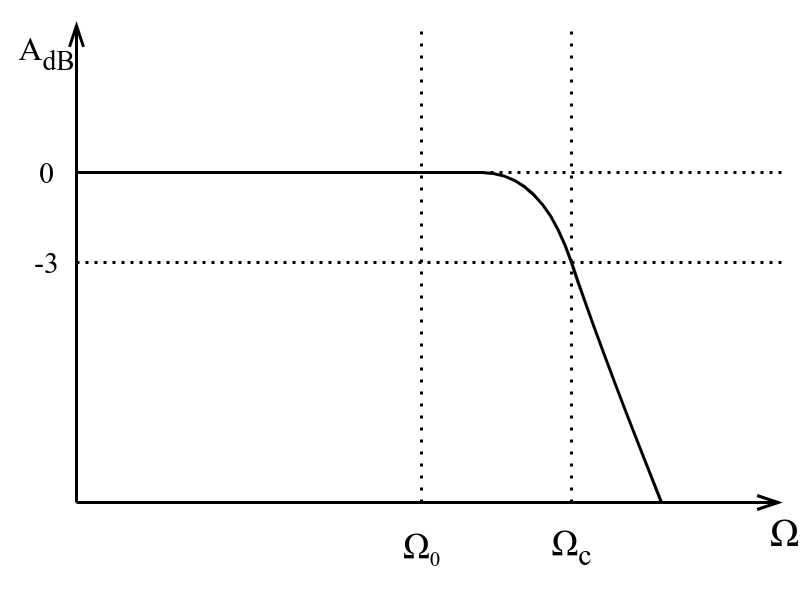
\includegraphics[width=300pt]{images/diagramas-bode-filtro-lp.png}
  \caption{Respuesta en frecuencia de un filtro pasa-bajos}
  \label{fig:diagrama_bode_pasa_bajos}
\end{figure}

Según \cite{rabiner1995theory} existen dos enfoques distintos para el diseño de filtros digitales de tipo pasa-banda, pasa-alto y rechaza-banda. Estos enfoques se resumen en la Figura \ref{fig:enfoques_diseno}. Estos dos enfoques difieren en que la técnica 1 transforma un filtro de paso bajo analógico normalizado en otro filtro analógico que se puede digitalizar para obtener el filtro digital deseado, mientras que la técnica 2 digitaliza el filtro de paso bajo normalizado inmediatamente y luego aplica una transformación de banda de frecuencia digital para obtener el filtro digital deseado. Dado que ya hemos discutido cómo diseñar el filtro de paso bajo normalizado y cómo digitalizarlo, en esta sección consideraremos las transformaciones de banda de frecuencia apropiadas para los casos continuo y discreto. Para nuestro diseño vamos a considerar la técnica 1, que consiste en pasar el filtro prototipo pasa-bajos a un pasa-banda para luego digitalizarlo utilizando la transformación bilineal.

\begin{figure}[H]
  \centering
  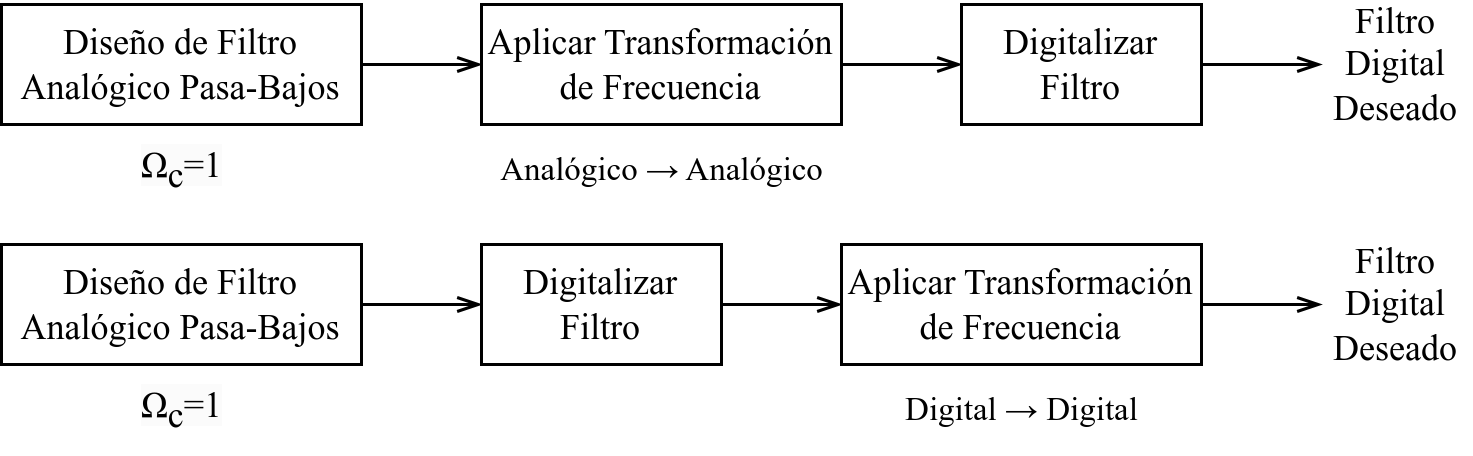
\includegraphics[width=\linewidth]{images/diagramas-enfoques-diseno.drawio.png}
  \caption{Enfoques para el diseño de un filtro digital}
  \label{fig:enfoques_diseno}
\end{figure}

Existe una gran variedad de técnicas para transformar un filtro pasa-bajas de corte 1 rad/s en otro filtro pasa-bajas (con diferente \gls{fc}) o en un filtro pasa-banda, pasa-altas o pasa-banda. A continuación se presenta un conjunto de transformaciones especialmente sencillas.

\begin{align}
  s & \rightarrow \frac{s}{\Omega_h}                                     & \textrm{pasa-bajos} \rightarrow \textrm{pasa-bajos}                           \\
  s & \rightarrow \frac{\Omega_l}{s}                                     & \textrm{pasa-bajos} \rightarrow \textrm{pasa-altos}                           \\
  s & \rightarrow \frac{s^2 + \Omega_l \Omega_h}{s(\Omega_h - \Omega_l)} & \textrm{pasa-bajos} \rightarrow \textrm{pasa-banda} \label{eq:transf_frec_pb} \\
  s & \rightarrow \frac{s(\Omega_h - \Omega_l)}{s^2 + \Omega_l \Omega_h} & \textrm{pasa-bajos} \rightarrow \textrm{rechaza-banda}                        \\
    &                                                                    & \Omega_l : \textrm{\gls{fc} inferior} \notag                                  \\
    &                                                                    & \Omega_h : \textrm{\gls{fc} superior} \notag
\end{align}

Cómo en este diseño vamos a utilizar la transformación de un pasa-bajos a un pasa-banda utilizaremos la Ecuación \ref{eq:transf_frec_pb}. Para utilizar el método, necesitamos establecer las frecuencias intervinientes: \gls{fc} superior e inferior, que las calculamos a partir de la elección de una frecuencia central. Para ello tomamos la frecuencia baja de los digitos 1, 2 y 3 (697 [Hz], Cuadro \ref{tab:combinacion_tonos}) que resulta ser la frecuencia más baja del espectro de este dominio. Las frecuencias de corte serán 60 [Hz] por encima y por debajo de la frecuencia central. Recordemos que para utilizar la transformación bilineal necesitamos compensar la distorsion de frecuencia, y para ello debemos realizar el pre-warping. Entonces las frecuencias angulares de corte analógicas superior e inferior estan dadas por la Ecuación \ref{eq:pre_warping_superior} y la Ecuación \ref{eq:pre_warping_inferior} respectivamente, donde \gls{fs} es igual a 44 [kHz].

\begin{equation}
  \Omega_h = 2 f_s \tan \left(\pi\frac{f_c+60}{f_s}\right) = 4761,01\ \mathrm{\left[\frac{rad}{s}\right]}
  \label{eq:pre_warping_superior}
\end{equation}

\begin{equation}
  \Omega_l = 2 f_s \tan \left(\pi\frac{f_c-60}{f_s}\right) = 4005,15\ \mathrm{\left[\frac{rad}{s}\right]}
  \label{eq:pre_warping_inferior}
\end{equation}

El siguiente paso es encontrar función transferencia realizando la transformación de frecuencia antes mencionada. En la Ecuación \ref{eq:func_transf_analog_reduc} podemos ver variables nuevas: $BW$ (\textit{Band-Width} o Ancho de Banda) y $\Omega_0$ que es la media geométrica del ancho de banda ($\sqrt{\Omega_h\Omega_l}$). Hacemos este reemplazo por motivos de simplicidad y para tener una mejor comprensión de la función transferencia.

\begin{align}
  H_{LP}(s) & = H_{BP}\left(\frac{s^2 + \Omega_l \Omega_h}{s(\Omega_h - \Omega_l)}\right)                                                                                  \\
  H(s)      & = \frac{1}{\frac{s^2 + \Omega_l \Omega_h}{s(\Omega_h - \Omega_l)}+1}                                                                                         \\
  H(s)      & = \frac{(\Omega_h - \Omega_l)s}{s^2 + (\Omega_h - \Omega_l)s + \Omega_h \Omega_l} = \frac{BW s}{s^2 + BW s + \Omega_0^2} \label{eq:func_transf_analog_reduc} \\
  H(s)      & = \frac{755,85 s}{s^2 + 755,85s + 19,07 \times 10^6}                                                                                                         \\
  H(s)      & = \frac{s}{0,00132s^2 + s + 25220}
\end{align}

Para demostrar que este filtro diseñado es en realidad un pasa-banda que corta en las frecuencias angulares especificadas, utilizamos MATLAB para graficar la respuesta en frecuencia del mismo (Código \ref{code:respuesta_freq_analog}). En la Figura \ref{fig:respuesta_freq_analog} podemos ver que la respuesta en frecuencia es la esperada, en los puntos marcados aproximadamente en y(0,707) las frecuencias se aproximan a $\Omega_l$ y $\Omega_h$. Por lo tanto queda demostrado que el filtro analógico diseñado es realmente un pasa-banda.

\lstinputlisting[
  language=Octave,
  caption={Graficar respuesta en frecuencia de Filtro Analógico},
  label={code:respuesta_freq_analog}
]{matlab/butter_analog_frec_resp.m}

\begin{figure}[H]
  \centering
  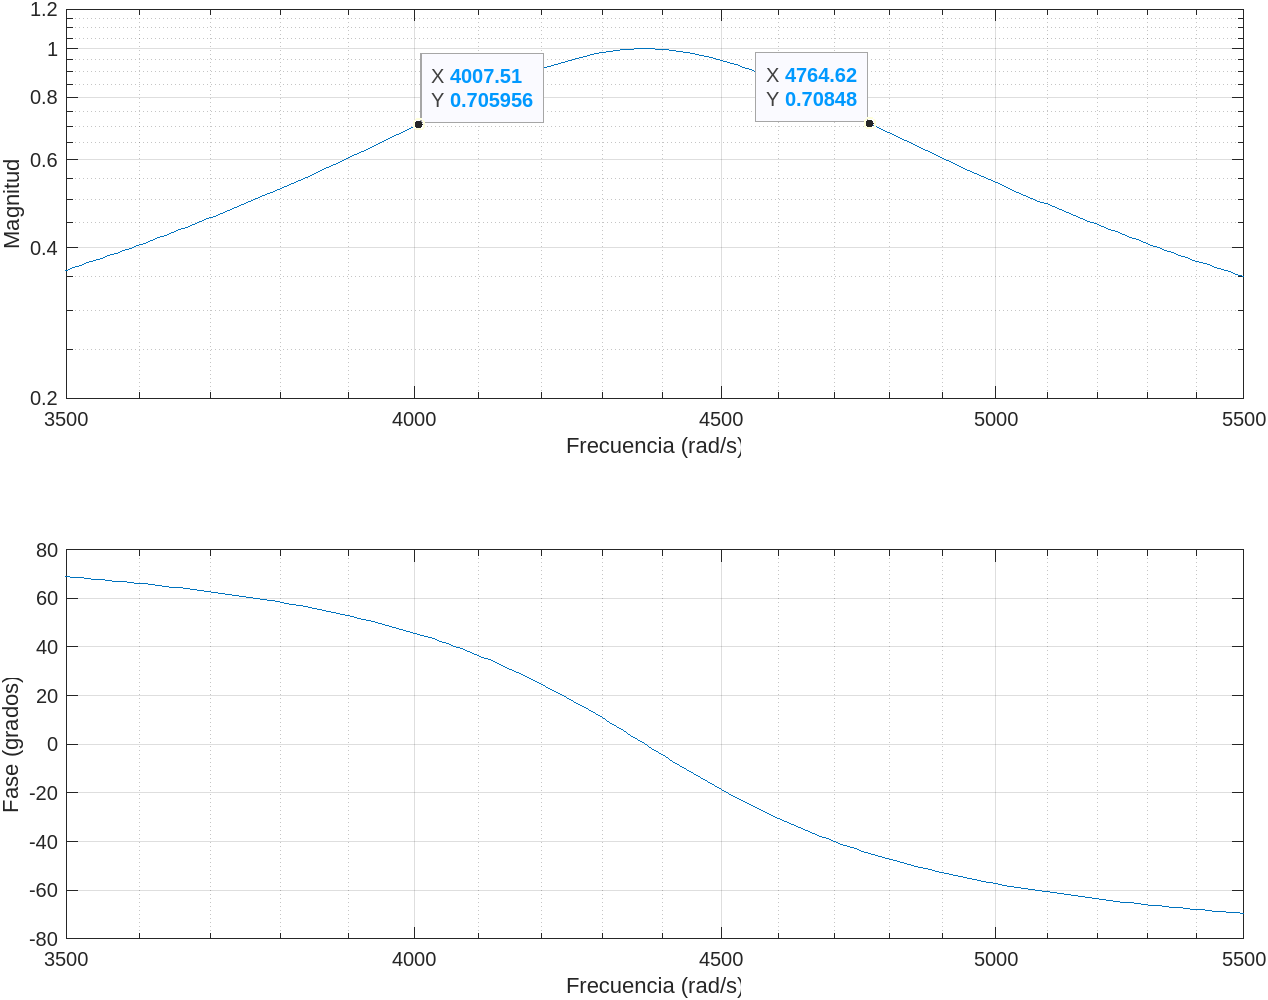
\includegraphics[width=\linewidth]{images/respuesta_frecuencia_analog.png}
  \caption{Respuesta en frecuencia del filtro analógico}
  \label{fig:respuesta_freq_analog}
\end{figure}

\section{Conversión a digital}
Ahora que tenemos nuestro filtro analógico, el siguiente paso es transformarlo a digital a tarvés de la Transformación Bilineal. Para realizarla consideramos la correspondencia entre el plano s y el plano z, dada por la Ecuación \ref{eq:transf_s_a_z}. Luego particularizamos la función transferencia de nuestro filtro pasa-banda analógico para la correspondencia antes mencionada, trabajamos algebráicamente (ver Apéndice \ref{eq:apendix_filtro_digital}) y encontramos H(z), que está dado por la Ecuación \ref{eq:filtro_digital_bp}.

\begin{align}
  s             & = \frac{2}{T}\frac{(1-\textrm{z}^{-1})}{(1+\textrm{z}^{-1})} \label{eq:transf_s_a_z}                                                                                                                                                                     \\
  H(\textrm{z}) & = H(s)|_{s = \frac{2}{T}\frac{(1-\textrm{z}^{-1})}{(1+\textrm{z}^{-1})}}                                                                                                                                                                                 \\
  H(\textrm{z}) & = \frac{BW \left(\frac{2}{T}\frac{(1-\textrm{z}^{-1})}{(1+\textrm{z}^{-1})}\right)}{\left(\frac{2}{T}\frac{(1-\textrm{z}^{-1})}{(1+\textrm{z}^{-1})}\right)^2 + BW \left(\frac{2}{T}\frac{(1-\textrm{z}^{-1})}{(1+\textrm{z}^{-1})}\right) + \Omega_0^2} \\
  H(\textrm{z}) & = \frac{8,49\times 10^{-3} - 8,49\times 10^{-3}\textrm{z}^{-2}}{1 - 1,97\textrm{z}^{-1} + 0,98\textrm{z}^{-2}} \label{eq:filtro_digital_bp}
\end{align}

Para demostrar que el filtro digital resultante funciona correctamente, utilizamos MATLAB para graficar la respuesta en frecuencia del mismo (ver Código \ref{code:respuesta_freq_digital}). En la Figura \ref{fig:respuesta_freq_digital} podemos ver que la respuesta en frecuencia es la esperada. En los puntos marcados aproximadamente en y(0,707) las frecuencias se aproximan a $f_l$ y $f_h$, que eran 60 [Hz] por debajo y por encima respectivamente de la frecuencia central 697 [Hz].

\lstinputlisting[
  language=Octave,
  caption={Graficar respuesta en frecuencia de Filtro Digital},
  label={code:respuesta_freq_digital}
]{matlab/butter_digital_frec_resp.m}

\begin{figure}[H]
  \centering
  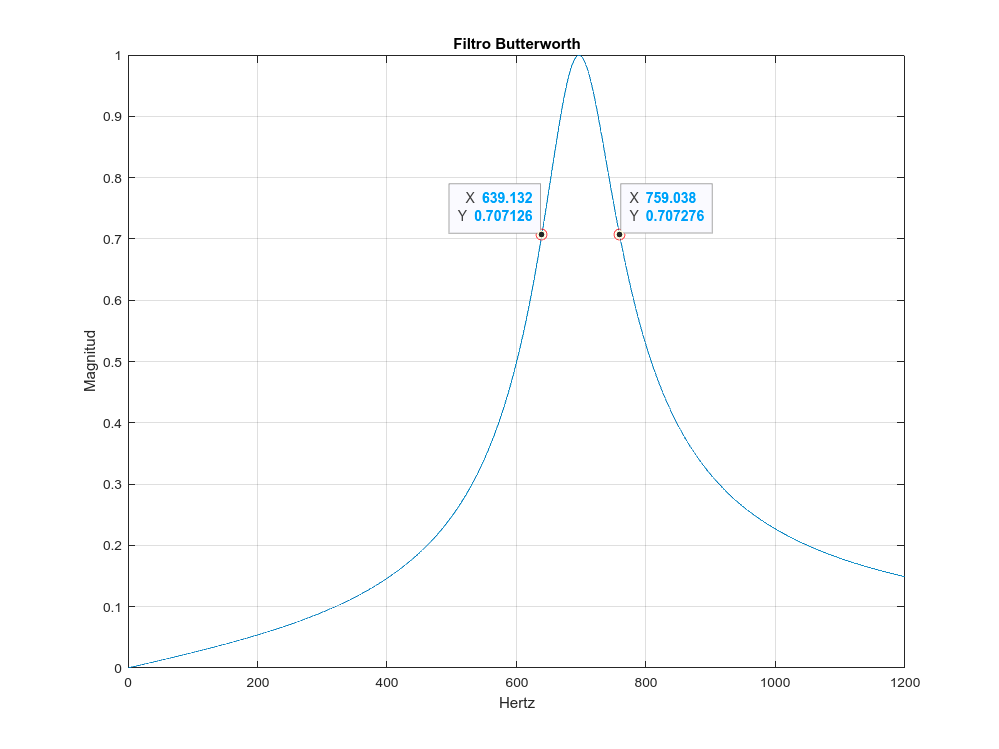
\includegraphics[width=\linewidth]{images/respuesta_frecuencia_digital.png}
  \caption{Respuesta en frecuencia del filtro digital}
  \label{fig:respuesta_freq_digital}
\end{figure}

\section{Conclusiones}
En las secciones anteriores demostramos cómo es el procedimiento para el diseño de un filtro digital pasa-banda a partir de transfomaciones aplicadas a un filtro analógico pasa-bajos. Analizamos las respectivas respuestas en frecuencia de los filtros analógicos y digitales obtenidos, y podemos observar que cumplen con el requisito de filtrar aquellas frecuencias que se encuentren fuera de la banda especificada [637 [Hz] ; 757 [Hz]]. Sin embargo este proceso fue solamente para un filtro, una banda de frecuencia para una frecuencia central en particular que es la primera del espectro de la matriz \gls{dtfm}. La siguiente frecuencia en el espectro es 770 [Hz], y si observamos la Figura \ref{fig:respuesta_freq_digital} podemos ver que no está muy lejos de la \gls{fc} superior del filtro diseñado. Esto va a devenir en un solapamiento de señales, lo cual puede introducir falsos disparos a la hora de implementar la lógica para detectar el tono. Queda claro que se necesita un filtro pasa-banda pero de mayor orden y una banda más reducida. El objetivo es definir un \gls{fa} superior e inferior, y en las que el filtro atenúe en 10 [dB], y estas frecuencias tienen que ser antes de solapar con la frecuencia siguiente o anterior del espectro de la matriz. En la Figura \ref{fig:diagrama_bode_pasa_banda} podemos ver cómo sería un filtro ideal pasa-banda que cumple con esos requisitos.

\begin{figure}[H]
  \centering
  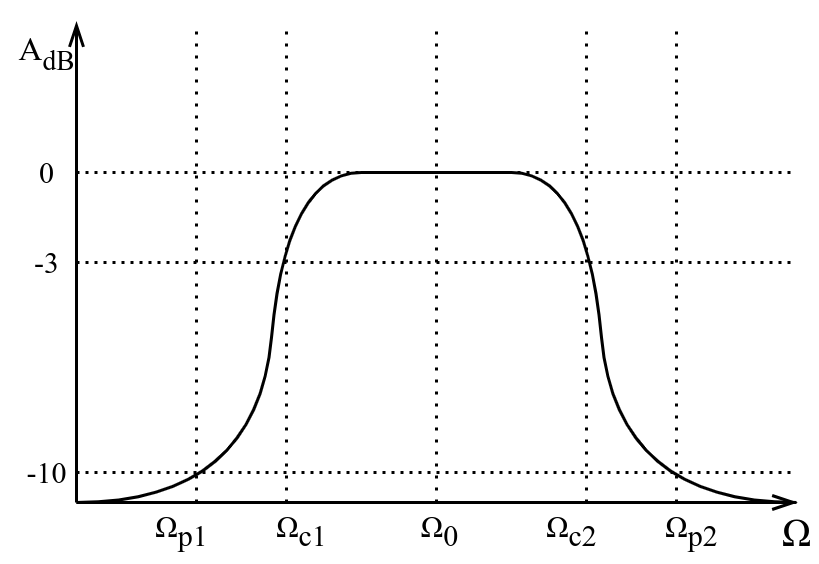
\includegraphics[width=300pt]{images/diagramas-bode-filtro-bp-mejorado.png}
  \caption{Respuesta en frecuencia de un filtro pasa-banda con frecuencias de parada}
  \label{fig:diagrama_bode_pasa_banda}
\end{figure}

Podemos calcular el orden del filtro pasa-bajo necesario para cumplir con esas características, luego sabremos que el filtro pasa-banda resultante será el doble de ese orden. Pero antes debemos definir las frecuencias críticas involucradas. A diferencia del filtro anterior, vamos a definir \gls{fc} 40 [Hz] por encima de la frecuencia central 697 [Hz], y luego \gls{fa} será 20 [Hz] por encima de \gls{fc}. Pero estas frecuencias son digitales, debemos calcularlas con la distorsión de la Transformación Bilineal (Pre-Warping) para resolver el orden. En las Ecuaciones \ref{eq:omega_c_analog} y \ref{eq:omega_a_analog} podemos ver las frecuencias analógicas resultantes. Luego, establecemos que la atenuación al final de la banda de transición y comienzo de la banda de rechazo (en \gls{fa}) es de 10 [dB]. Con estos datos podemos obtener el orden mínimo para que se requiere para el filtro pasa-bajos analógico. De la Ecuación \ref{eq:orden_filtro_pb} vemos que el valor es 41, que es mucho mayor que el orden 1 que utilizamos en el diseño a partir del filtro prototipo.

\begin{align}
  \Omega_c & = \frac{2}{T} \tan \frac{\omega_c T}{2} = 2 f_s \tan\left(\pi \frac{f_c}{f_s}\right) = 4634,99 \mathrm{\left[\frac{rad}{s}\right]} \label{eq:omega_c_analog} \\
  \Omega_a & = \frac{2}{T} \tan \frac{\omega_a T}{2} = 2 f_s \tan\left(\pi \frac{f_a}{f_s}\right) = 4761,01 \mathrm{\left[\frac{rad}{s}\right]} \label{eq:omega_a_analog} \\
  n        & = \frac{\log\left(10^{\frac{A_{dB}}{10}-1}\right)}{2\log\left(\frac{\Omega_a}{\Omega_c}\right)} = 40,95 \approx 41 \label{eq:orden_filtro_pb}
\end{align}

Con esto demostramos y concluímos que para obtener un filtro más preciso en la simulación, necesitamos que sea de mayor orden. Dado que el análisis es engorroso y debemos repetirlo por cada filtro del banco de filtros a diseñar, vamos a utilizar una herramienta de MATLAB llamada fdatool para obtener el filtro digital con el orden necesario para obtener los resultados esperados a partir de las especificaciones realizadas.
